
%
%%----------------------------------------------------------------

\newpage
\section{Modelo de información: Módulo Academias}
\subsection{Descripción general}
%En la figura~\ref{fig:asistenciaAlumno} se muestra la estructura de información que manejará el proceso de ejecución de periodo escolar.

%\begin{figure}[htbp!]
%	\begin{center}
%		\fbox{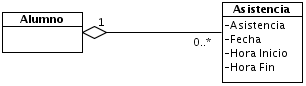
\includegraphics[width=.5\textwidth]{images/clases/AsistenciaAlumnos.png}}
%		\caption{Modelo de información del proceso de Instituciones para Movilidad.}
%		\label{fig:asistenciaAlumno}
%	\end{center}
%\end{figure}

%--------------------------------------------------------------------------------
\begin{BusinessEntity}{academia}{Academia}
	
	\Battr{nombre}{Nombre}{\tdFrase}{Es el nombre con el que se registra la academia}{\requerido}{\longitudMax{100}{caracteres}}{Caracteres admitidos: [A-Z] $|$ [a-z] $|$ \textvisiblespace.}

\end{BusinessEntity}


%--------------------------------------------------------------------------------